\documentclass[tikz,border=8pt]{standalone}
% Shared look for every TikZ diagram. Load with % Shared look for every TikZ diagram. Load with % Shared look for every TikZ diagram. Load with \input{../../tools/tikz-style.tex}
\usepackage[T1]{fontenc}
\usepackage{lmodern}
\renewcommand{\sfdefault}{lmr}  % diagrams use the same serif as the text
\usetikzlibrary{arrows.meta, positioning, shapes.geometric, calc, fit, backgrounds}
\definecolor{cblue}{HTML}{4C78A8}
\definecolor{corange}{HTML}{F58518}
\definecolor{cgreen}{HTML}{54A24B}
\definecolor{cred}{HTML}{E45756}
\definecolor{cpurple}{HTML}{B279A2}
\definecolor{cgrey}{HTML}{6B6B6B}
\tikzset{
  every picture/.style={font=\sffamily, line width=1.2pt},
  box/.style={draw=#1, fill=#1!12, rounded corners=4pt, align=center, inner sep=7pt, minimum height=1.1cm},
  box/.default=cgrey,
  arrow/.style={-{Stealth[length=3mm]}, draw=cgrey, line width=1.4pt},
  title/.style={font=\sffamily\bfseries\Large},
  note/.style={font=\sffamily\small, text=cgrey, align=center},
}
\AtBeginDocument{\hyphenpenalty=10000 \exhyphenpenalty=10000}

\usepackage[T1]{fontenc}
\usepackage{lmodern}
\renewcommand{\sfdefault}{lmr}  % diagrams use the same serif as the text
\usetikzlibrary{arrows.meta, positioning, shapes.geometric, calc, fit, backgrounds}
\definecolor{cblue}{HTML}{4C78A8}
\definecolor{corange}{HTML}{F58518}
\definecolor{cgreen}{HTML}{54A24B}
\definecolor{cred}{HTML}{E45756}
\definecolor{cpurple}{HTML}{B279A2}
\definecolor{cgrey}{HTML}{6B6B6B}
\tikzset{
  every picture/.style={font=\sffamily, line width=1.2pt},
  box/.style={draw=#1, fill=#1!12, rounded corners=4pt, align=center, inner sep=7pt, minimum height=1.1cm},
  box/.default=cgrey,
  arrow/.style={-{Stealth[length=3mm]}, draw=cgrey, line width=1.4pt},
  title/.style={font=\sffamily\bfseries\Large},
  note/.style={font=\sffamily\small, text=cgrey, align=center},
}
\AtBeginDocument{\hyphenpenalty=10000 \exhyphenpenalty=10000}

\usepackage[T1]{fontenc}
\usepackage{lmodern}
\renewcommand{\sfdefault}{lmr}  % diagrams use the same serif as the text
\usetikzlibrary{arrows.meta, positioning, shapes.geometric, calc, fit, backgrounds}
\definecolor{cblue}{HTML}{4C78A8}
\definecolor{corange}{HTML}{F58518}
\definecolor{cgreen}{HTML}{54A24B}
\definecolor{cred}{HTML}{E45756}
\definecolor{cpurple}{HTML}{B279A2}
\definecolor{cgrey}{HTML}{6B6B6B}
\tikzset{
  every picture/.style={font=\sffamily, line width=1.2pt},
  box/.style={draw=#1, fill=#1!12, rounded corners=4pt, align=center, inner sep=7pt, minimum height=1.1cm},
  box/.default=cgrey,
  arrow/.style={-{Stealth[length=3mm]}, draw=cgrey, line width=1.4pt},
  title/.style={font=\sffamily\bfseries\Large},
  note/.style={font=\sffamily\small, text=cgrey, align=center},
}
\AtBeginDocument{\hyphenpenalty=10000 \exhyphenpenalty=10000}

\begin{document}
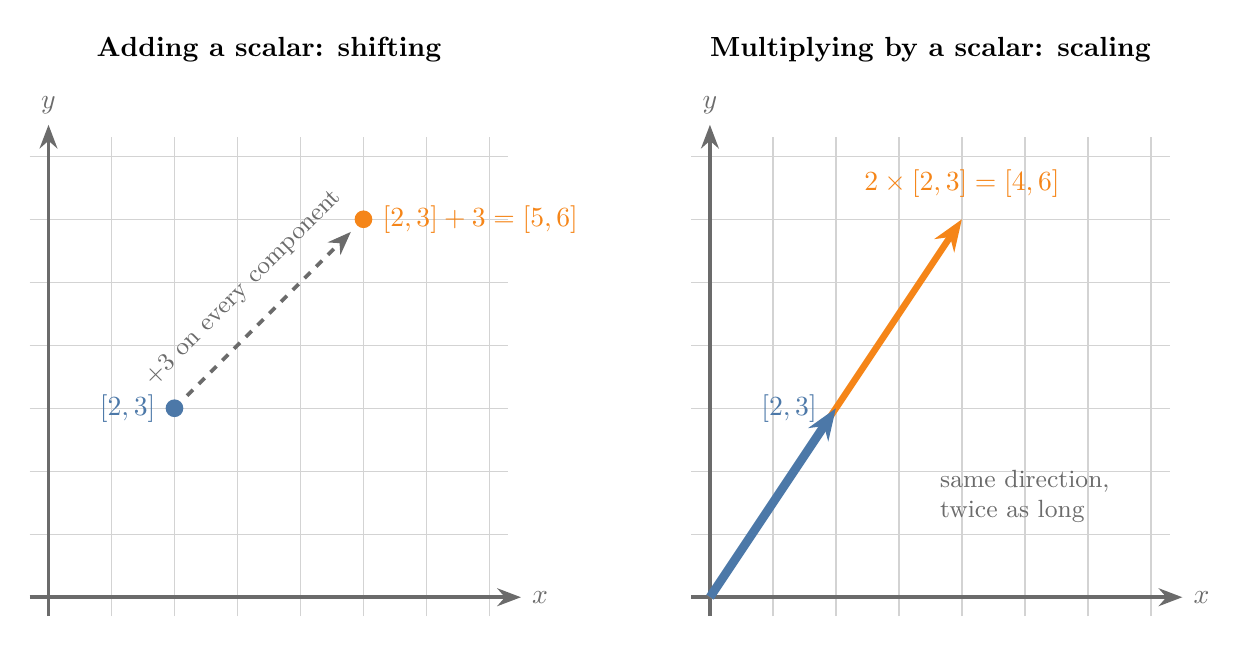
\begin{tikzpicture}[scale=0.8]
  \begin{scope}
    \node[font=\bfseries] at (3.5,8.7) {Adding a scalar: shifting};
    \draw[cgrey!30, line width=0.5pt] (-0.3,-0.3) grid (7.3,7.3);
    \draw[arrow, cgrey] (-0.3,0) -- (7.5,0) node[right] {$x$};
    \draw[arrow, cgrey] (0,-0.3) -- (0,7.5) node[above] {$y$};
    \fill[cblue] (2,3) circle (4pt) node[left=3pt, text=cblue, font=\bfseries] {$[2,3]$};
    \fill[corange] (5,6) circle (4pt) node[right=3pt, text=corange, font=\bfseries] {$[2,3]+3=[5,6]$};
    \draw[arrow, dashed] (2.2,3.2) -- (4.8,5.8);
    \node[note, rotate=45] at (3.1,4.9) {+3 on every component};
  \end{scope}
  \begin{scope}[xshift=10.5cm]
    \node[font=\bfseries] at (3.5,8.7) {Multiplying by a scalar: scaling};
    \draw[cgrey!30, line width=0.5pt] (-0.3,-0.3) grid (7.3,7.3);
    \draw[arrow, cgrey] (-0.3,0) -- (7.5,0) node[right] {$x$};
    \draw[arrow, cgrey] (0,-0.3) -- (0,7.5) node[above] {$y$};
    \draw[-{Stealth[length=4mm]}, corange, line width=2.4pt] (0,0) -- (4,6);
    \draw[-{Stealth[length=4mm]}, cblue, line width=3.2pt] (0,0) -- (2,3);
    \node[left=3pt, text=cblue, font=\bfseries] at (2,3) {$[2,3]$};
    \node[above=4pt, text=corange, font=\bfseries] at (4,6) {$2 \times [2,3] = [4,6]$};
    \node[note, align=left] at (5.0,1.6) {same direction,\\ twice as long};
  \end{scope}
\end{tikzpicture}
\end{document}
